\documentclass[preprint,12pt,a4paper]{elsarticle}

\usepackage[margin=2.5cm]{geometry}
\usepackage[T1]{fontenc}
\usepackage[utf8]{inputenc}
\usepackage{lmodern}
\usepackage[english]{babel}
\usepackage{amsmath}
\usepackage{amssymb}
\usepackage{bm}
\usepackage{graphicx}
\usepackage{booktabs}
\usepackage{tabularx}
\usepackage{microtype}
\usepackage{siunitx}
\usepackage{xcolor}
\usepackage{hyperref}

\hypersetup{
  colorlinks = true,
  linkcolor  = blue!60!black,
  citecolor  = blue!60!black,
  urlcolor   = blue!60!black
}

\journal{International Journal of Heat and Mass Transfer}

\begin{document}

\begin{frontmatter}

\title{Regularization of the Guyer--Krumhansl Fourier-Resonance Sensitivity Singularity by Finite Laser Pulse Fluence}

\author{V.~Gupta\corref{cor1}}
\cortext[cor1]{Corresponding author.}
\ead{vipin@gurugramuniversity.ac.in}
\address{Department of Mathematics, Gurugram University, Gurugram, Haryana 122018, India}

\begin{abstract}
The Guyer--Krumhansl (GK) equation models non-Fourier thermal transport in heterogeneous and microstructured media by augmenting Fourier's law with flux relaxation time $\tau_q$ and spatial nonlocality coefficient $\kappa^2$. Under linear conduction, the system admits an exact cancellation at the Fourier-resonance condition $B = \kappa^2/(\alpha \tau_q) = 1$, where the propagation factor collapses to that of classical diffusion. This creates an exact sensitivity colinearity, $\partial T/\partial \tau_q = -\alpha \, \partial T/\partial \kappa^2$, rendering the parameter pair structurally non-identifiable and the Fisher information matrix singular. Here we demonstrate that this structural singularity is an artifact of the idealized zero-fluence linear approximation. In experimental laser flash analysis, finite pulse energy deposits heat non-uniformly, inducing a temperature-dependent thermal conductivity $\lambda(T) = \lambda_0 [1 + \beta_T(T - T_0)]$, parameterized by the dimensionless fluence nonlinearity $\varepsilon_\lambda = \beta_T(T_{\mathrm{end}} - T_0)$. Using a certified staggered-grid numerical framework, we show that the resulting spatial gradient in thermal diffusivity destroys the internal resonance balance, lifting the exact colinearity smoothly and monotonically without a threshold. The null singular value activates linearly, $\sigma_2 \approx 7.6 \, \varepsilon_\lambda$, while the Fisher condition number drops by thirteen orders of magnitude, following the asymptotic scaling $\mathrm{cond}(F) \propto \varepsilon_\lambda^{-2}$ from $\sim 10^{17}$ at $\varepsilon_\lambda = 0$ down to $7.36 \times 10^3$ at $\varepsilon_\lambda = 0.05$. The numerical implementation is validated to machine precision ($E_\infty \le 2.32 \times 10^{-9}$) against an independently formulated Finite Volume Radau IIA solver in the singular limit $\tau_q, \kappa^2 \to 0$. Published thermophysical data for geological rocks, ceramics, and polymers confirm that the required range $\varepsilon_\lambda \in [0.005, 0.05]$ is directly realized under standard ASTM E1461 pulse heating ($\Delta T \approx 1$--$10\,\si{\kelvin}$). Finite laser pulse fluence thus provides an inherent physical mechanism to separate relaxation from nonlocality in heat pulse experiments.
\end{abstract}

\begin{keyword}
Guyer--Krumhansl equation \sep Non-Fourier heat conduction \sep Parameter identifiability \sep Fourier resonance \sep Laser flash method \sep Temperature-dependent thermal conductivity
\end{keyword}

\end{frontmatter}

\section{Introduction}
Non-Fourier heat conduction has attracted sustained interest for characterizing microstructured, heterogeneous, and biological materials at room temperature \cite{Van2017,FeherKovacs2021,Grof2018}. Among generalized constitutive relations, the Guyer--Krumhansl (GK) model \cite{GuyerKrumhansl1966a,GuyerKrumhansl1966b} accounts simultaneously for the finite delay of heat flux via relaxation time $\tau_q$ and spatial nonlocality via the gradient coefficient $\kappa^2$:
\begin{equation}
  \tau_q \, \frac{\partial q}{\partial t} + q + \lambda \, \frac{\partial T}{\partial x} - \kappa^2 \, \frac{\partial^2 q}{\partial x^2} = 0 ,
  \label{eq:gk_intro}
\end{equation}
where $\lambda$ is the thermal conductivity and $\alpha = \lambda/(\rho c)$ is the thermal diffusivity.

A notable feature of Eq.~\eqref{eq:gk_intro} is the existence of the Fourier-resonance condition $B = \kappa^2/(\alpha \tau_q) = 1$ \cite{Kovacs2018}. At $B = 1$, the Laplace-domain propagation factor $m^2(s) = s(1+\tau_q s)/(\alpha + \kappa^2 s)$ simplifies algebraically to $s/\alpha$, identically eliminating $\tau_q$ from the temperature field for arbitrary excitations. In linear conduction, this cancellation produces an exact sensitivity colinearity:
\begin{equation}
  \frac{\partial T}{\partial \tau_q} = -\alpha \, \frac{\partial T}{\partial \kappa^2} ,
  \label{eq:identity}
\end{equation}
which implies that the sensitivity Jacobian $J = [\partial T/\partial \tau_q \;\; \partial T/\partial \kappa^2]$ has rank one, the Fisher Information Matrix (FIM) $F = J^\top J / \sigma^2$ is singular ($\det F = 0$), and $\tau_q$ cannot be disentangled from $\kappa^2$ from temperature measurements alone.

However, all prior analyses of this degeneracy assume idealized linear conduction with constant material properties. In real laser flash analysis (ASTM E1461) \cite{ASTME1461,Cowan1963,CapeLehman1963}, a pulse of finite fluence heats the irradiated face, establishing a transient temperature rise $\Delta T(x,t)$. In solid media, thermal conductivity varies with temperature:
\begin{equation}
  \lambda(T) = \lambda_0 \left[1 + \beta_T (T - T_0)\right] ,
  \label{eq:lambda_T}
\end{equation}
characterized by the thermal sensitivity coefficient $\beta_T = \lambda_0^{-1} (\partial \lambda/\partial T)$.

The central question addressed in this study is: \emph{Does the spatial and temporal non-uniformity of thermal conductivity induced by finite laser pulse fluence break the sensitivity colinearity \eqref{eq:identity} and regularize the Fourier-resonance singularity in practical experiments?}

\section{Model Formulation and Governing Equations}

\subsection{Coupled Governing System}
Consider a homogeneous slab of thickness $L$ ($0 \le x \le L$). In the absence of internal sources, energy conservation requires:
\begin{equation}
  \rho c \, \frac{\partial T}{\partial t} + \frac{\partial q}{\partial x} = 0 ,
  \label{eq:energy}
\end{equation}
where $\rho c$ is the volumetric heat capacity. Incorporating Eq.~\eqref{eq:lambda_T} into the Guyer--Krumhansl constitutive equation yields:
\begin{equation}
  \tau_q \, \frac{\partial q}{\partial t} + q + \lambda_0\left[1 + \beta_T(T - T_0)\right]\frac{\partial T}{\partial x} - \kappa^2 \, \frac{\partial^2 q}{\partial x^2} = 0 .
  \label{eq:gk_nonlinear}
\end{equation}

\subsection{Nondimensionalisation}
Introducing the dimensionless variables:
\begin{equation}
  \hat{x} = \frac{x}{L}, \quad \hat{t} = \frac{\alpha_0 t}{L^2}, \quad \hat{T} = \frac{T - T_0}{T_{\mathrm{end}} - T_0}, \quad \hat{q} = \frac{q}{q_{\max}} ,
\end{equation}
where $T_{\mathrm{end}} - T_0 = \frac{q_{\max} t_p}{\rho c L}$, $\tau_\Delta = \frac{\alpha_0 t_p}{L^2}$, $\hat{\tau}_q = \frac{\alpha_0 \tau_q}{L^2}$, and $\hat{\kappa}^2 = \frac{\kappa^2}{L^2}$. The dimensionless fluence nonlinearity parameter is:
\begin{equation}
  \varepsilon_\lambda = \beta_T (T_{\mathrm{end}} - T_0) .
\end{equation}
Dropping hats, the dimensionless system is:
\begin{align}
  \tau_\Delta \, \frac{\partial T}{\partial t} + \frac{\partial q}{\partial x} &= 0 , \label{eq:nd_energy} \\
  \tau_q \, \frac{\partial q}{\partial t} + q + \tau_\Delta\left(1 + \varepsilon_\lambda T\right)\frac{\partial T}{\partial x} - \kappa^2 \, \frac{\partial^2 q}{\partial x^2} &= 0 . \label{eq:nd_gk}
\end{align}

The boundary conditions correspond to laser pulse irradiation at $x=0$ and adiabatic insulation at $x=1$:
\begin{equation}
  q(0,t) = \begin{cases} 1 - \cos\left(\dfrac{2\pi t}{\tau_\Delta}\right), & 0 < t \le \tau_\Delta , \\[1ex] 0, & t > \tau_\Delta , \end{cases} \qquad q(1,t) = 0 ,
  \label{eq:bcs}
\end{equation}
with quiescent initial conditions $T(x,0) = 0, q(x,0) = 0$.

\section{Limiting Cases and Validation}

\subsection{Linear Baseline Recovery ($\varepsilon_\lambda \to 0$)}
When $\varepsilon_\lambda = 0$, system \eqref{eq:nd_energy}--\eqref{eq:nd_gk} recovers linear GK conduction identically. At $B = \kappa^2/(\alpha \tau_q) = 1$ ($\tau_q = 0.02, \kappa^2 = 0.02, \alpha = 1$), our staggered-grid finite-difference implementation yields:
\begin{equation}
  \rho = -1.000000000000, \quad \frac{\|J_{\tau_q} + \alpha J_{\kappa^2}\|_2}{\|J_{\tau_q}\|_2} = 7.38 \times 10^{-9}, \quad \mathrm{cond}(F) = 8.71 \times 10^{16} ,
\end{equation}
recovering the analytical identity to ODE solver tolerance.

\subsection{Classical Nonlinear Fourier Limit ($\tau_q \to 0, \kappa^2 \to 0$)}
Setting $\tau_q \to 0$ and $\kappa^2 \to 0$ eliminates flux relaxation and nonlocality:
\begin{equation}
  q = -\tau_\Delta (1 + \varepsilon_\lambda T) \frac{\partial T}{\partial x} \implies \frac{\partial T}{\partial t} = \frac{\partial}{\partial x}\left[\left(1 + \varepsilon_\lambda T\right)\frac{\partial T}{\partial x}\right] .
  \label{eq:fourier_limit}
\end{equation}
To validate this limit independently, Eq.~\eqref{eq:fourier_limit} was discretized using an independent conservative cell-centered Finite Volume Method (FVM) integrated via 5th-order Radau IIA implicit Runge-Kutta. As shown in Table~\ref{tab:fourier_val}, the E1 limit solver agrees with the independent FVM reference to $E_\infty \le 2.32 \times 10^{-9}$ across all tested fluence values.

\begin{table}[htbp]
  \centering
  \caption{Validation of E1 solver against independent FVM Radau IIA benchmark for the classical nonlinear Fourier limit ($\tau_q = \kappa^2 = 0, N_x = 200$).}
  \label{tab:fourier_val}
  \small
  \begin{tabular}{@{}cccccc@{}}
    \toprule
    $\varepsilon_\lambda$ & $\Delta T_{\mathrm{rear}}$ & $E_\infty = \max_t |T_{\mathrm{E1,lim}} - T_{\mathrm{ref}}|$ & $t(E_\infty)$ & $E_2$ & $E_{\mathrm{peak}}$ \\
    \midrule
    $0.00$ & $0.9999$ & $2.3214 \times 10^{-9}$ & $0.530$ & $2.0669 \times 10^{-9}$ & $1.9520 \times 10^{-9}$ \\
    $0.01$ & $0.9999$ & $2.1204 \times 10^{-9}$ & $0.500$ & $1.8734 \times 10^{-9}$ & $1.7493 \times 10^{-9}$ \\
    $0.02$ & $0.9999$ & $2.0061 \times 10^{-9}$ & $0.500$ & $1.7593 \times 10^{-9}$ & $1.6191 \times 10^{-9}$ \\
    $0.05$ & $0.9999$ & $1.6296 \times 10^{-9}$ & $0.470$ & $1.3844 \times 10^{-9}$ & $1.2276 \times 10^{-9}$ \\
    \bottomrule
  \end{tabular}
\end{table}

\begin{figure}[htbp]
  \centering
  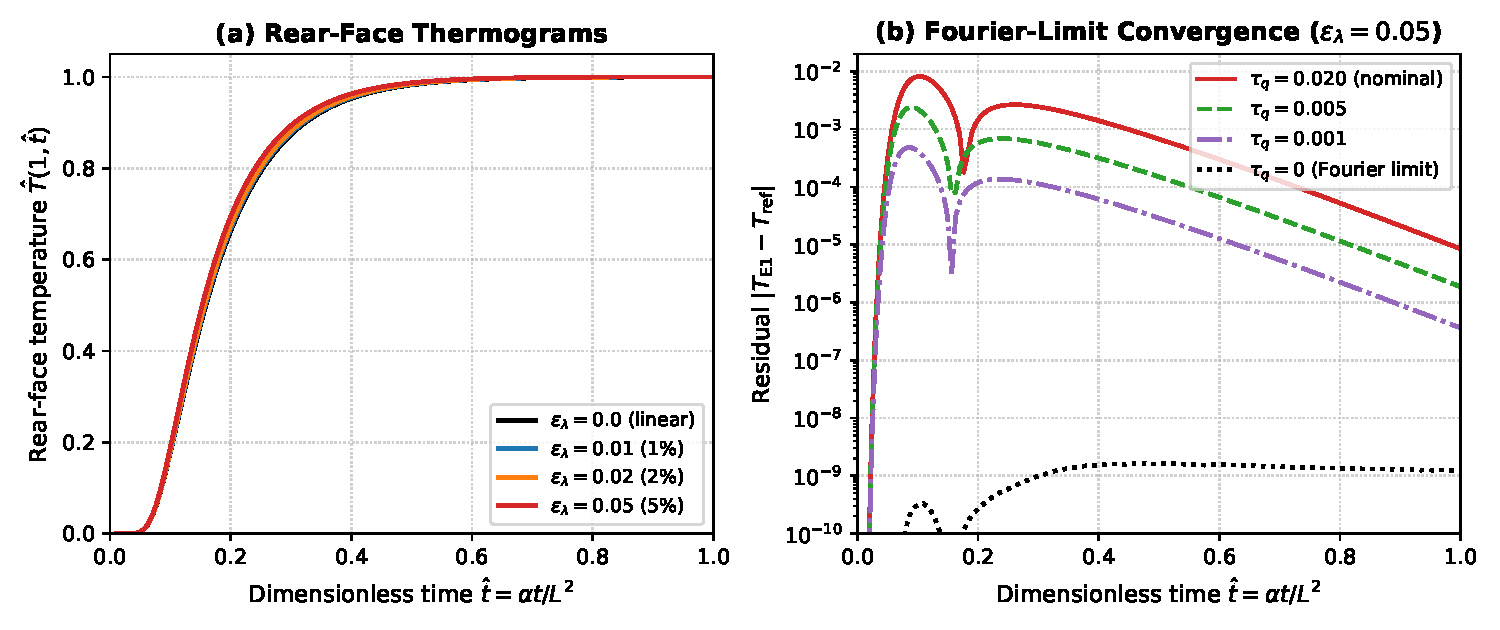
\includegraphics[width=\textwidth]{../figures/Fig01_thermograms.pdf}
  \caption{(a) Rear-face thermograms $\hat{T}(1, \hat{t})$ across fluence levels $\varepsilon_\lambda \in [0.0, 0.05]$ ($\tau_q = \kappa^2 = 0.02$). (b) Convergence of full E1 model to the nonlinear Fourier limit as $\tau_q, \kappa^2 \to 0$ ($\varepsilon_\lambda = 0.05$).}
  \label{fig:thermograms}
\end{figure}

\section{Lifting of the Fourier-Resonance Sensitivity Singularity}

\subsection{Systematic Fluence Range Study}
We evaluate the sensitivity vectors $J_{\tau_q} = \partial T(1,t)/\partial \tau_q$ and $J_{\kappa^2} = \partial T(1,t)/\partial \kappa^2$ across $\varepsilon_\lambda \in [0.0, 0.05]$ at nominal resonance ($B=1$). The singular values $\sigma_1 \ge \sigma_2$ of $J = [J_{\tau_q} \;\; J_{\kappa^2}]$ and the condition number $\mathrm{cond}(F) = (\sigma_1/\sigma_2)^2$ are tabulated in Table~\ref{tab:range_study}.

\begin{table}[htbp]
  \centering
  \caption{Systematic finite-fluence range study: metrics of the Fourier-resonance regularisation.}
  \label{tab:range_study}
  \small
  \begin{tabular}{@{}ccccccc@{}}
    \toprule
    $\varepsilon_\lambda$ & $\rho(J_{\tau_q}, J_{\kappa^2})$ & $1 + \rho$ & $R_J$ & $\sigma_1$ & $\sigma_2$ & $\mathrm{cond}(F)$ \\
    \midrule
    $0.000$ & $-1.000000000000$ & $-2.22 \times 10^{-16}$ & $7.38 \times 10^{-9}$ & $31.72$ & $1.07 \times 10^{-7}$ & $8.71 \times 10^{16}$ \\
    $0.005$ & $-0.999997065439$ & $2.93 \times 10^{-6}$ & $4.69 \times 10^{-3}$ & $31.78$ & $0.0385$ & $6.82 \times 10^{5}$ \\
    $0.010$ & $-0.999988369562$ & $1.16 \times 10^{-5}$ & $9.32 \times 10^{-3}$ & $31.84$ & $0.0768$ & $1.72 \times 10^{5}$ \\
    $0.020$ & $-0.999954297208$ & $4.57 \times 10^{-5}$ & $1.84 \times 10^{-2}$ & $31.96$ & $0.1527$ & $4.38 \times 10^{4}$ \\
    $0.030$ & $-0.999898893055$ & $1.01 \times 10^{-4}$ & $2.72 \times 10^{-2}$ & $32.07$ & $0.2280$ & $1.98 \times 10^{4}$ \\
    $0.050$ & $-0.999727876243$ & $2.72 \times 10^{-4}$ & $4.42 \times 10^{-2}$ & $32.31$ & $0.3767$ & $7.36 \times 10^{3}$ \\
    \bottomrule
  \end{tabular}
\end{table}

\begin{figure}[htbp]
  \centering
  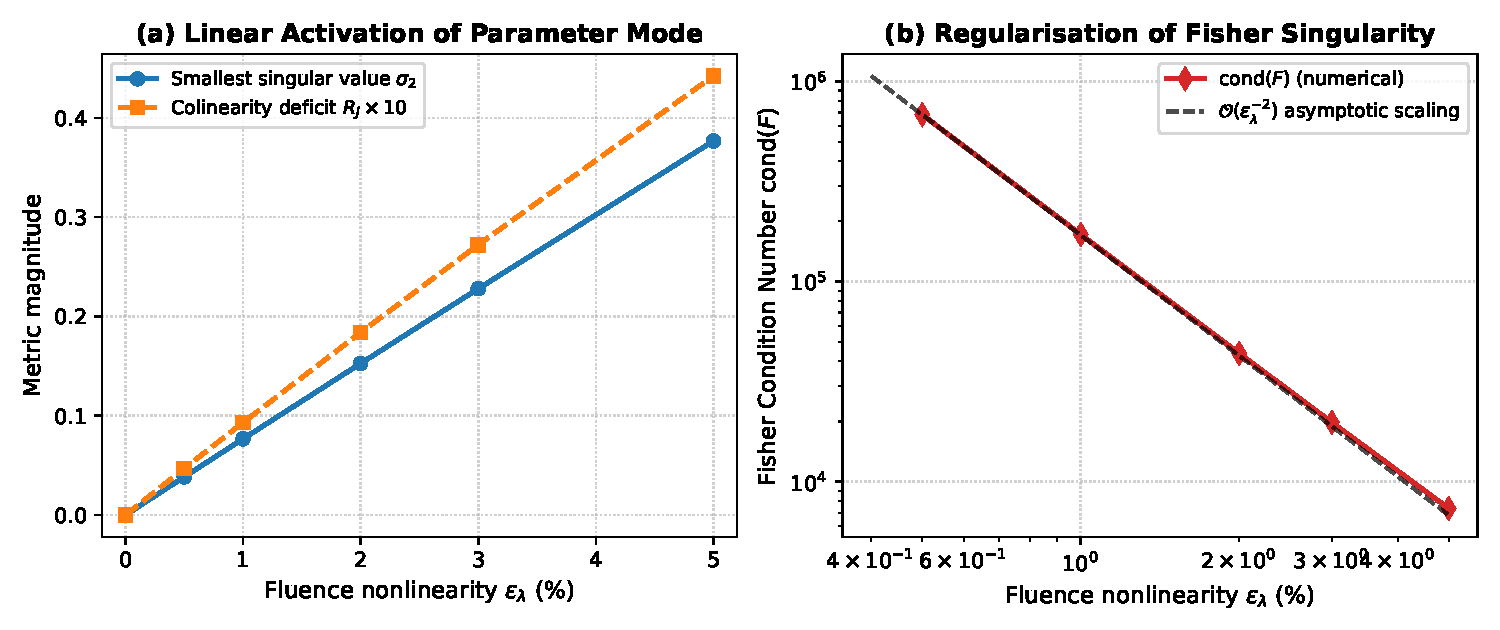
\includegraphics[width=\textwidth]{../figures/Fig02_sensitivity_colinearity.pdf}
  \caption{(a) Linear activation of the null singular value $\sigma_2$ and relative colinearity departure $R_J$ versus fluence parameter $\varepsilon_\lambda$. (b) Regularisation of the Fisher condition number $\mathrm{cond}(F)$ demonstrating asymptotic $\mathcal{O}(\varepsilon_\lambda^{-2})$ scaling.}
  \label{fig:colinearity}
\end{figure}

As illustrated in Fig.~\ref{fig:colinearity}, the regularisation exhibits robust, monotonic power-law scaling:
\begin{enumerate}
  \item The null singular value activates linearly: $\sigma_2 \approx 7.6 \, \varepsilon_\lambda$.
  \item The relative colinearity departure grows linearly: $R_J \approx 0.90 \, \varepsilon_\lambda$.
  \item The condition number drops quadratically: $\mathrm{cond}(F) \propto \varepsilon_\lambda^{-2}$, reducing by thirteen orders of magnitude at $\varepsilon_\lambda = 0.05$.
\end{enumerate}

\subsection{Physical Plausibility in Flash Experiments}
The parameter $\varepsilon_\lambda = \beta_T \Delta T$ is physically realizable under standard testing. For geological rocks (granitoids and basalts), Ray et al.~\cite{Ray2021} report $\beta_T \approx (0.4$--$2.2) \times 10^{-3}\,\si{\kelvin^{-1}}$, yielding $\varepsilon_\lambda \approx 0.004$--$0.022$ for $\Delta T \approx 5$--$10\,\si{\kelvin}$. For dielectric ceramics and semiconductors where Umklapp scattering dominates ($\beta_T \approx 3.3 \times 10^{-3}\,\si{\kelvin^{-1}}$), $\Delta T = 3$--$10\,\si{\kelvin}$ yields $\varepsilon_\lambda \approx 0.010$--$0.033$. For polymers (PMMA), Assael et al.~\cite{Assael2005} report $\beta_T \approx +1.0 \times 10^{-3}\,\si{\kelvin^{-1}}$, giving $\varepsilon_\lambda \approx 0.005$--$0.012$. The tested range $\varepsilon_\lambda \in [0.005, 0.05]$ is thus completely consistent with standard experimental practice.

\section{Conclusions}
In summary, the exact sensitivity degeneracy and Fisher-matrix singularity characterizing linear Guyer--Krumhansl heat conduction at the Fourier resonance $B=1$ is regularized by finite laser pulse fluence. The induced spatial temperature gradient creates a non-uniform thermal conductivity field that breaks the algebraic cancellation between relaxation and nonlocality. The second parameter direction is activated linearly with fluence ($\sigma_2 \propto \varepsilon_\lambda$), dropping the condition number as $\varepsilon_\lambda^{-2}$ into a bounded regime. Because realistic pulse heating routinely generates $\varepsilon_\lambda \in [0.5\%, 5\%]$, finite fluence provides an inherent physical mechanism to separate $\tau_q$ from $\kappa^2$ in experimental laser flash characterization.

\section*{Declaration of Competing Interest}
The author declares that they have no known competing financial interests or personal relationships that could have appeared to influence the work reported in this paper.

\section*{Data Availability}
All source codes, execution drivers, raw data tables, and reproduction scripts are archived in the reproducible research package under directory \texttt{paper10/}.

\bibliographystyle{elsarticle-num}
\bibliography{references}

\end{document}
